\subsection{Microbiota dataset}

As we look into the microbiota data, we notice a major phylogenetic architecture to describe various levels of precision in the microbiota composition.
Indeed, such phylogenetic structure can be represented as a tree as on the following figure:
\begin{figure}[H]
    \center
    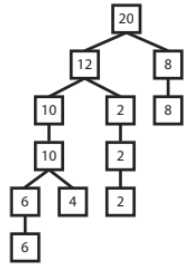
\includegraphics[scale=1]{images/abundance_tree_phylogenetic}
    \caption{Phylogenetic tree example with abundance data (in the nodes) at each layer of the tree.
    Each node represents a bacterium specie at a given precision layer in the tree. From \cite{microbiome_deeplearning_research}.}
    \label{fig:phylogenetic_tree}
\end{figure}

Such structure can not be used directly in a machine learning system since it's not a vectorizable representation.
Hence, we first suggest to transform the tree in a matrix to image structure as in the following example:
\begin{figure}[H]
    \center
    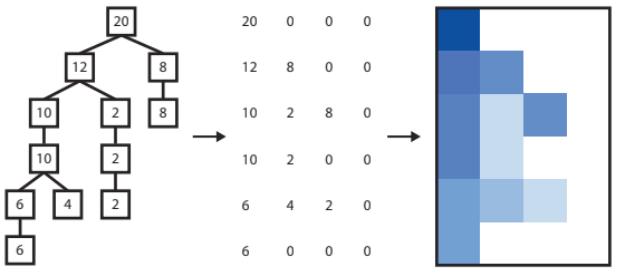
\includegraphics[scale=1]{images/tree_to_image}
    \caption{Phylogenetic tree to image representation:
    opacity of the pixel relates to the abundance of the species at the given level of precision (normalized between 0 and 1).
    From \cite{microbiome_deeplearning_research}.}
    \label{fig:phylogenetic_tree_to_img}
\end{figure}

To give some notations, we introduce the following framework:
\begin{itemize}
    \item The maximum depth of a phylogenetic tree is $D$, the maximum number of nodes $N_T$, and the maximum amount of unique species at any level is $U$.
    \item $X_i$ is the abundance matrix of the individual $i$ (image of size $D \times U$) , which is observed.
    \item $T_i$ is the adjacent matrix of the phylogenetic tree of individual $i$, of size $N_T \times N_T$, which is observed.
    We could use any other encoding of a tree (contour function, depth function, $\dots$).
    \item We assume that we have $n$ individuals observed through $(X_i, T_i)_{1 \leq i \leq n}$ i.i.d samples.
\end{itemize}
